\documentclass[11pt,letterpaper]{article}

\usepackage[utf8]{inputenc}
\usepackage[T1]{fontenc}
\usepackage{amsmath,amssymb,amsthm,mathtools}
\usepackage{graphicx}
\usepackage{hyperref}
\usepackage{geometry}
\usepackage{float}
\usepackage{tikz}
\usetikzlibrary{arrows.meta,calc,positioning,shapes.geometric,decorations.pathmorphing,patterns,fit,backgrounds}
\usepackage{pgfplots}
\pgfplotsset{compat=1.18}
\usepackage{booktabs}
\usepackage[numbers,sort&compress]{natbib}
\usepackage{xcolor}
\usepackage{tcolorbox}
\usepackage{enumitem}
\usepackage{bm}
\usepackage{array}
\usepackage{multirow}
% \usepackage{microtype} % disabled: font expansion unavailable in this TeX Live
% siunitx not available in this TeX Live; manual unit macros
\newcommand{\microwatt}{\ensuremath{\mu\mathrm{W}}}
\newcommand{\micrometreSq}{\ensuremath{\mu\mathrm{m}^2}}

\geometry{margin=1in}
\graphicspath{{figures/convergence/}{figures/processor/}{figures/}}

\tcbuselibrary{skins,breakable}

% Okabe--Ito palette
\definecolor{oiOrange}{HTML}{E69F00}
\definecolor{oiSky}{HTML}{56B4E9}
\definecolor{oiGreen}{HTML}{009E73}
\definecolor{oiYellow}{HTML}{F0E442}
\definecolor{oiBlue}{HTML}{0072B2}
\definecolor{oiVerm}{HTML}{D55E00}
\definecolor{oiPurple}{HTML}{CC79A7}

\hypersetup{colorlinks=true,linkcolor=oiBlue,citecolor=oiVerm,urlcolor=oiBlue}

% Hypothesis box
\newtcolorbox{hypothesis}[1]{%
  colback=oiSky!8, colframe=oiBlue!80!black,
  fonttitle=\bfseries, title={#1},
  breakable, enhanced, sharp corners=south}

% Non-claim box
\newtcolorbox{nonclaim}{%
  colback=oiVerm!8, colframe=oiVerm!80!black,
  fonttitle=\bfseries, title={What is \emph{not} claimed},
  breakable, enhanced, sharp corners=south}

% Locked-identity shorthand
\newcommand{\gzero}{g_0}
\newcommand{\Evac}{E_{\mathrm{vac}}}
\newcommand{\Flock}{F}
\newcommand{\lastar}{\lambda^{\!\star}}
\newcommand{\lfold}{\lambda_{\mathrm{fold}}}
\newcommand{\AresAc}{A^{\!\star}\!/A_c}
\newcommand{\Qhopf}{Q_H}
\newcommand{\Tstar}{T^{\!\star}}
\newcommand{\aH}{a_H}
\newcommand{\Dstar}{\Delta^{\!\star}}
\newcommand{\Dzero}{\Delta_0}

\newtheorem{definition}{Definition}

\title{%
  Convergence Hypotheses for a Topological Condensed-Matter Processor:\\[4pt]
  \large Nine Cross-Discipline Predictions from Fractal Circuits, Vacuum-Field Effects,\\
  Hopfion Topology, and Floquet Metamaterials}

\author{Mineral Hoiland}
\date{August 2026 \quad --- \quad \textsc{L1/L2 only; L3 quarantined}}

\begin{document}
\maketitle

% ============================================================
\begin{abstract}
We derive nine new labeled hypotheses for the TDVT topological processor by synthesising established experimental paradigms---Josephson junction array (JJA) vortex lattices, cavity-mediated vacuum coherence in graphene, static hopfions in chiral magnets, magnomechanical phonon lasers, graphene fractal plasmonic metamaterials, structured-vacuum light-by-light scattering, optical-cavity vacuum magnetic birefringence, and fractal Floquet topological insulators---with the locked identities of the Quantum Vacuum Catalyzation (QVC) framework.
Every hypothesis carries a falsifier, a fabrication stage, and a quantitative prediction tied to the Option~A$^{\!\star}$ parameter set ($\gzero = 0.0982$~meV, $\Evac = 0.1287$~meV, $\Flock = 0.58068$, $\lastar = 0.7628$, $\AresAc = 0.9117$, $\theta = \pi/10$, $\Qhopf = 1/N$, $\Tstar = 118.7$~mK).
Approximately half of the framework builds on established physics (Devil's staircase in JJAs since Halsey 1985, DCE since Wilson 2011, integer Hopf charge since Kent 2021); the remainder---catalyzon quasiparticle concept, fractional Hopf charge, OAM structure in DCE photons, Helmert decomposition of JJA modes, vacuum-pumped multi-mode phonon lasing---is genuinely novel.
All predictions remain on L1 (algebra/transport) and L2 (lab-constructable devices); L3 spacetime ontology is quarantined.
\end{abstract}

\tableofcontents

% ============================================================
\section{Introduction}\label{sec:intro}

The TDVT topological processor is a proposed superconducting--van~der~Waals device stack whose mathematical backbone rests on three objects: a democratic coupling matrix $G = \gzero(J - I)$ whose spectrum partitions into one bright eigenvalue $\lambda_{\max} = (N{-}1)\gzero$ and an $(N{-}1)$-fold dark Helmert subspace at $\lambda_{\min} = -\gzero$; a saddle-node fold map $\delta = 1 + \alpha(\ln\delta + \ell)$ that controls the gap $\Delta(A,\lambda)$; and a Chern--Simons fractional Hopf charge $\Qhopf = 1/N$ with abelian exchange $\theta = \pi/(2N)$ on the lens space $L(N,1)$.
The processor paper~\cite{ProcessorPaper} develops device hypotheses H-DARK1 through H-MCM1 from the locked Option~A$^{\!\star}$ identities and three fabrication roadmap reviews~\cite{Xin2022,Pham2022,Dobrovolskiy2026}.

This companion note asks a different question: what happens when nine additional experimental paradigms---each probing vacuum-field effects, topological charge, fractal geometry, or circuit QED---are mapped onto the same locked parameter set?
The answer is ten new hypotheses that extend the processor stack without touching L3 (spacetime ontology, Einstein $G$, or universal TQC).

The nine source papers span eight orders of magnitude in energy ($10^{-5}$--$10^3$~meV) and five in length ($10^{-1}$--$10^4$~nm).
Despite this range, every locked TDVT parameter has at least one experimental counterpart in the source literature (Fig.~\ref{fig:energy}).
The Josephson energy $E_J \approx 0.107$~meV measured by Cosmic et al.\ in an aluminium JJA~\cite{Cosmic2018} sits within 9\% of $\gzero = 0.0982$~meV.
The helical wavelength $\lambda_h \approx 70$~nm of FeGe hopfions~\cite{Tai2018} is $1.4\times$ the coherence length $\xi = 50$~nm.
The fractal Floquet edge states of Yang et al.~\cite{Yang2020} and Li et al.~\cite{Li2023} demonstrate topological protection on non-translational (Sierpi\'{n}ski) lattices with real-space Chern number $C = 1$ and $2^N$ exponential state-space scaling.
The cavity vacuum birefringence sensitivity of $1.8 \times 10^{-17}$~m/$\sqrt{\text{Hz}}$ achieved by Spector et al.~\cite{Spector2026} proves that quantum-vacuum structure is experimentally accessible at the required precision.
Bu et al.~\cite{Bu2026} show that vortex lasers with OAM $\ell = \pm 10$ imprint topological phase on vacuum-polarised photons---precisely the OAM quantum number $\ell = 2N = 10$ that the processor's CS level $k = 2N$ would assign.

What follows is a systematic derivation of nine hypotheses from these convergences.

\begin{figure}[t]
  \centering
  \includegraphics[width=\textwidth]{fig_energy_convergence.pdf}
  \caption{\textbf{Energy-scale convergence.}
  Horizontal bars mark the locked TDVT identities ($\gzero$, $\Evac$, $4\gzero$, $\Dstar$, $\Dzero$).
  Coloured markers show where the nine source papers sit.
  The Josephson energy $E_J \approx 0.107$~meV of the JJA (Cosmic et al.) falls within 9\% of $\gzero = 0.0982$~meV; the FeGe exchange energy $J_{\mathrm{ex}} \approx 0.6$~meV per bond (Tai \& Smalyukh) matches $\Dzero = 0.600$~meV.
  }\label{fig:energy}
\end{figure}


% ============================================================
\section{Locked Identities (Option A$^{\!\star}$)}\label{sec:locks}

All predictions in this note use the frozen fat-torus geometry $(r,R) = (8,50)$~nm with the following parameter set.  No value may be adjusted to fit a new hypothesis; any prediction that contradicts a lock falsifies the hypothesis, not the lock.

\begin{table}[H]
\centering
\caption{Option A$^{\!\star}$ locked identities.}\label{tab:locks}
\begin{tabular}{@{}lrl@{}}
\toprule
\textbf{Quantity} & \textbf{Value} & \textbf{Status} \\
\midrule
$\Flock = \sum K_0(nx)$               & $0.58068$           & locked \\
$\Evac = \frac{1}{4\pi^2}\frac{\hbar c_s}{r}\Flock$ & $0.1287$~meV  & locked \\
$\lfold$                                & $0.8475$            & locked \\
$\lastar = 0.90\,\lfold$               & $0.7628$            & locked \\
$\Dstar$                                & $0.2324$~meV        & locked \\
$\gzero = \lastar\Evac$                 & $0.0982$~meV        & locked \\
$\lambda_{\max} = (N{-}1)\gzero$        & $0.3928$~meV ($N{=}5$) & derived \\
$\lambda_{\min} = -\gzero$ (mult.\ $N{-}1$) & $-0.0982$~meV & derived \\
$\lambda_{\max}/\lambda_{\min}$          & $-4$                & scale-free \\
$\Qhopf = 1/N$                          & $0.2$ ($N{=}5$)     & locked \\
$k = 2N$                                & $10$ ($N{=}5$)      & locked \\
$\theta = \pi/(2N)$                      & $\pi/10$            & abelian \\
$\delta\sigma_{xy} = e^2/(2Nh)$         & $e^2/(10h) \approx 3.874 \times 10^{-6}$~S & locked \\
$\AresAc$                               & $0.9117$ (resonant) & locked \\
$\Tstar$                                & $118.7$~mK          & Schwinger \\
\bottomrule
\end{tabular}
\end{table}

\begin{nonclaim}
This note does not claim: (i)~QVC observed in the laboratory; (ii)~Einstein gravity recovered from hopfion crystals (H-EIN1/2 fail); (iii)~$\theta = \pi/10$ enables universal topological quantum computation (abelian braiding only); (iv)~$\Tstar = 118.7$~mK is a Hawking temperature (it is a Schwinger diagnostic from $E_{\mathrm{pair}} = 2|\gzero|$); (v)~$\Evac/h \approx 31.1$~GHz is a ``detection'' of $\Evac$ (band coincidence with 32~GHz bolometers, not a measurement); (vi)~any L3 spacetime ontology.
\end{nonclaim}


% ============================================================
\section{Hypothesis H-JJA1: Commensurate Vortex Lattice at $f = 1/5$}\label{sec:hjja1}

\subsection{Source convergence}
Cosmic et al.~\cite{Cosmic2018} measure a 30$\times$3 aluminium JJA at $E_J/h = 25.8$~GHz ($E_J \approx 0.107$~meV) in a 3D copper cavity (TE$_{101}$, 10.127~GHz, $\kappa/2\pi \approx 100$~MHz).  They observe commensurate vortex lattice states at fractional flux fillings $\Phi/\Phi_0 = 0, 1/9, 1/6, 1/3, 1/2, 2/3, 5/6, 1$.
The filling $f = 1/5$ was not measured but lies within the accessible range.

The TDVT processor uses $N = 5$ islands with democratic coupling $\gzero = 0.0982$~meV.  The proximity of $E_J$ and $\gzero$ ($< 9\%$ discrepancy) means the same JJA hardware, tuned by junction area or critical current, sits at the TDVT energy scale.

\subsection{Prediction}

\begin{hypothesis}{H-JJA1: Commensurate vortex lattice at $f = 1/5$}
\textbf{Setup.}  A 5$\times$3 aluminium JJA with $E_J$ tuned to $\gzero = 0.0982$~meV (junction area $\sim 4 \times 4$~$\mu$m$^2$), coupled to a 3D cavity at $\omega_c/2\pi \approx 10$~GHz, frustrated at $\Phi/\Phi_0 = 1/5$.

\textbf{Prediction.}  The cavity reflection spectrum $S_{11}(\omega)$ exhibits a mode structure with:
\begin{equation}\label{eq:jja1_split}
  \frac{\omega_{\mathrm{bright}} - \omega_c}{\omega_{\mathrm{dark}} - \omega_c}
  = \frac{\lambda_{\max}}{\lambda_{\min}}
  = -(N{-}1) = -4,
\end{equation}
where $\omega_{\mathrm{bright}}$ is the single superradiant plasma mode and $\omega_{\mathrm{dark}}$ are the $(N{-}1) = 4$ dark (subradiant) modes.
The plasma frequency of the bright mode is shifted by $\chi_{\mathrm{bright}} = (N{-}1)\gzero/\hbar \approx 4 \times 23.75$~GHz from the bare cavity, while each dark mode shifts by $\chi_{\mathrm{dark}} = -\gzero/\hbar \approx -23.75$~GHz.

At $f = 1/5$, the vortex lattice is commensurate with the 5-plaquette unit cell.  The critical current at this filling obeys:
\begin{equation}
  I_c(f{=}1/5) = I_{c,0}\,\Flock \cdot \left|\cos\!\left(\frac{\pi}{5}\right)\right| = I_{c,0} \times 0.58068 \times 0.80902,
\end{equation}
where $\Flock = 0.58068$ is the locked Bessel factor and $\cos(\pi/5)$ is the geometric frustration weight for a pentagonal unit cell.

\textbf{Falsifier.}  (a)~Mode ratio $\neq -4$ at $f = 1/5$; (b)~no commensurate state at $f = 1/5$; (c)~$I_c(f{=}1/5)$ inconsistent with $\Flock$.

\textbf{Stage.}  0 (Al/Nb JJA; existing circuit QED technology).
\end{hypothesis}


% ============================================================
\section{Hypothesis H-VH1: Vacuum-Harvested Dark Coherence}\label{sec:hvh1}

\subsection{Source convergence}
Dakir, Slaoui, and Ahl~Laamara~\cite{Dakir2026} show that cavity vacuum fluctuations mediate inter-layer quantum coherence in triple-layer graphene.  The relative entropy of coherence (REC) and tripartite tangle $\tau_g$ increase with the number of cavity modes $n_{\max}$ and peak at optimal interlayer spacing $d_i/L$.
Their system has $N = 3$ layers.  We ask: what happens at $N = 5$?

\subsection{Derivation}
For $N$ identical layers in a planar cavity, the vacuum-mediated coupling matrix is democratic: $G_{ij} = \gzero$ for $i \neq j$, $G_{ii} = 0$.  The Helmert transform decomposes the $N$-layer density matrix into one bright (centre-of-mass) channel and $(N{-}1)$ dark (relative) channels.

The total REC partitions as:
\begin{equation}\label{eq:rec_partition}
  \mathrm{REC}_{\mathrm{total}} = \mathrm{REC}_{\mathrm{bright}} + \sum_{k=1}^{N-1} \mathrm{REC}_{\mathrm{dark},k}.
\end{equation}
In the democratic limit, each dark channel carries equal coherence.  The ratio is:
\begin{equation}\label{eq:rec_ratio}
  \frac{\mathrm{REC}_{\mathrm{dark,total}}}{\mathrm{REC}_{\mathrm{bright}}}
  = \frac{(N{-}1) \cdot |\lambda_{\min}|^2}{|\lambda_{\max}|^2}
  = \frac{(N{-}1) \cdot \gzero^2}{[(N{-}1)\gzero]^2}
  = \frac{1}{N{-}1} = \frac{1}{4}.
\end{equation}
The bright channel dominates, but the dark subspace carries 20\% of the total vacuum-harvested coherence---protected from radiative decay by the subradiant eigenvalue structure.

\begin{hypothesis}{H-VH1: Vacuum-harvested dark coherence in $N$-layer cavity}
\textbf{Setup.}  Five graphene (or TMD) layers in a planar microcavity, interlayer spacing $d_i$ tuned so that the effective vacuum coupling matches $\lastar = 0.7628$.

\textbf{Prediction.}
\begin{enumerate}[nosep]
  \item The REC partitions into 1 bright $+$ 4 dark channels with $\mathrm{REC}_{\mathrm{dark}}/\mathrm{REC}_{\mathrm{bright}} = 1/4$.
  \item The non-Markovianity $\mathcal{N}_{\mathrm{REC}}$ peaks at $\lastar = 0.7628$ (the fold participation).
  \item The dark coherence lifetime exceeds the bright lifetime by the Purcell suppression factor $(N{-}1)^2 = 16$.
\end{enumerate}

\textbf{Falsifier.}  REC does not partition into Helmert channels; dark coherence vanishes; non-Markovianity monotonic in $\lambda$ (no peak at $\lastar$).

\textbf{Stage.}  3 (cavity-coupled vdW stack; extends H-VT1).
\end{hypothesis}


% ============================================================
\section{Hypothesis H-FRAC1: Fractal Devil's Staircase at $d_H = 3/4$}\label{sec:hfrac1}

\subsection{Source convergence}
De~Nicola et al.~\cite{DeNicola2020} fabricate Au/graphene Sierpi\'{n}ski-carpet photodetectors ($d_H = \ln 8/\ln 3 \approx 1.89$) with self-similar LSP resonances spanning VIS to MIR.  Yang et al.~\cite{Yang2020} and Li et al.~\cite{Li2023} demonstrate Floquet topological edge states on Sierpi\'{n}ski-gasket photonic lattices ($d_H = \ln 3/\ln 2 \approx 1.585$) with Chern $C = 1$ and $2^N$ exponential state scaling.

The TDVT processor predicts a Devil's staircase in $\sigma_{xy}(\mu)$ with Hausdorff dimension $d_H = 3/4$.  This is distinct from the literature value $d_H \approx 0.87$ measured in conventional JJA critical-current staircases~\cite{Halsey1985}.

\subsection{Derivation}
The Hall conductance staircase has plateaus at rational fillings $\nu = p/q$ (with $\gcd(p,q) = 1$) of width:
\begin{equation}\label{eq:plateau_width}
  w_{p/q} = \frac{e^2}{2Nh} \cdot \Flock \cdot q^{-1/d_H},
\end{equation}
where the Bessel factor $\Flock = 0.58068$ weights each plateau by the vacuum geometry and $d_H$ controls the scaling exponent.  The total measure of all plateaus in the interval $[0, e^2/h]$ is:
\begin{equation}
  \mu_{\mathrm{total}} = \sum_{p/q} w_{p/q} \propto \sum_{q=1}^{\infty} \varphi(q)\, q^{-1/d_H},
\end{equation}
where $\varphi(q)$ is Euler's totient.  For $d_H = 3/4$, the exponent $1/d_H = 4/3$ and the sum converges (the staircase is ``incomplete''---has positive-measure gaps, a Cantor-like complement).  For $d_H = 1$, the staircase is complete (Minkowski's question-mark function).

The number of resolvable plateaus at measurement resolution $\varepsilon$ scales as:
\begin{equation}\label{eq:nplateau}
  N_{\mathrm{plateau}}(\varepsilon) \sim \left(\frac{\varepsilon_{\max}}{\varepsilon}\right)^{d_H},
\end{equation}
with $\varepsilon_{\max} = e^2/h$.  At the pentamer resolution $\varepsilon = e^2/(2Nh) = e^2/(10h)$:
\begin{equation}
  N_{\mathrm{plateau}} = 10^{3/4} \approx 5.62,
\end{equation}
rounding to 5 or 6 addressable plateaus---matching the 5-island register plus the bright mode (Fig.~\ref{fig:staircase}).

\begin{figure}[t]
  \centering
  \includegraphics[width=0.85\textwidth]{fig_devils_staircase.pdf}
  \caption{\textbf{Devil's staircase.}  Solid blue: TDVT prediction $d_H = 3/4$.  Dashed grey: literature JJA value $d_H \approx 0.87$.  The TDVT staircase has wider gaps (less complete), yielding $N_{\mathrm{plateau}} \approx 5.6$ at the pentamer resolution $\varepsilon = e^2/(10h)$.
  }\label{fig:staircase}
\end{figure}

\begin{hypothesis}{H-FRAC1: Devil's staircase at $d_H = 3/4$}
\textbf{Setup.}  A JJA at $\gzero$ with flux sweep $\Phi/\Phi_0 \in [0,1]$; Hall bar or dispersive readout of $\sigma_{xy}$.

\textbf{Prediction.}  The staircase has $d_H = 3/4 = 0.75$, distinct from the established $d_H \approx 0.87$, and the fractal memory capacity is $N_{\mathrm{plateau}}(\varepsilon) = (\varepsilon_{\max}/\varepsilon)^{3/4}$.

\textbf{Falsifier.}  (a)~Box-counting gives $d_H \neq 0.75 \pm 0.05$; (b)~no staircase structure below $\Tstar$.

\textbf{Stage.}  1 (He-FIB JJA; extends H-SSH1 to 2D fractal response).
\end{hypothesis}


% ============================================================
\section{Hypothesis H-FFTI1: Floquet Topological SSH Shuttle}\label{sec:hffti1}

\subsection{Source convergence}
Yang et al.~\cite{Yang2020} demonstrate photonic Floquet topological insulators on a Sierpi\'{n}ski gasket with $C = 1$ and Li et al.~\cite{Li2023} achieve 100\% hopping efficiency via a 4-step driving protocol in a dual Sierpi\'{n}ski carpet, generating $2^N$ quantum states.

The TDVT SSH shuttle (H-SSH1) is a 1D chain with alternating hoppings $t_1, t_2$.  We propose that periodic (Floquet) cycling of the four dark Helmert modes converts the shuttle into a Floquet topological insulator whose topological gap and braid phase are locked to the processor identities.

\subsection{Derivation}
The 4-step driving protocol for $N = 5$ islands activates one dark-mode pair per step.  The single-period Floquet operator is:
\begin{equation}\label{eq:floquet_U}
  \hat{U}(T) = e^{-i H_4 T/4}\, e^{-i H_3 T/4}\, e^{-i H_2 T/4}\, e^{-i H_1 T/4},
\end{equation}
where each $H_k$ couples one Helmert pair $\{|h_k\rangle, |h_{k+1 \bmod 4}\rangle\}$ with strength $\gzero$.

The quasi-energy spectrum has a topological gap:
\begin{equation}\label{eq:floquet_gap}
  \Delta_F = \gzero \sin\!\left(\frac{\pi}{N}\right) = 0.0982 \times \sin\!\left(\frac{\pi}{5}\right) \approx 0.0577~\text{meV}.
\end{equation}
The edge state inside this gap accumulates a braid phase per cycle:
\begin{equation}\label{eq:braid_phase}
  \theta_{\mathrm{braid}} = \frac{\pi}{2N} = \frac{\pi}{10},
\end{equation}
which is exactly the locked abelian exchange angle.
The real-space Chern number is $C = 1$, computed by the same formula as Yang et al.\ applied to the non-translational fractal (Fig.~\ref{fig:floquet}).

\begin{figure}[t]
  \centering
  \includegraphics[width=0.85\textwidth]{fig_floquet_ssh.pdf}
  \caption{\textbf{Floquet SSH quasi-energy spectrum.}  Bulk bands (blue) separated by topological gap $\Delta_F \approx 0.0577$~meV.  Red star: edge state accumulating $\theta = \pi/10$ per cycle.
  }\label{fig:floquet}
\end{figure}

\begin{hypothesis}{H-FFTI1: Floquet topological SSH shuttle}
\textbf{Setup.}  H-SSH1 chain with 4-step periodic driving at frequency $\Omega = 2\pi/T$, where each step activates one dark-mode pair.

\textbf{Prediction.}
\begin{enumerate}[nosep]
  \item Topological gap $\Delta_F = \gzero\sin(\pi/N) \approx 0.0577$~meV.
  \item Accumulated braid phase $\theta = \pi/(2N) = \pi/10$ per cycle.
  \item Soliton transfer efficiency $\geq 90\%$ (topologically protected, as in Li et al.).
  \item Real-space Chern number $C = 1$.
\end{enumerate}

\textbf{Falsifier.}  (a)~No topological gap; (b)~$\theta \neq \pi/10$; (c)~soliton transfer $< 80\%$; (d)~$C \neq 1$.

\textbf{Stage.}  2 (SSH plaquette interferometer; extends H-SSH1).
\end{hypothesis}


% ============================================================
\section{Hypothesis H-OAM1: DCE Vortex Emission at $\ell = 2N$}\label{sec:hoam1}

\subsection{Source convergence}
Bu et al.~\cite{Bu2026} demonstrate that vortex lasers with OAM $\ell = \pm 10$ imprint topological phase on vacuum-polarised photons, enhancing light-by-light scattering by $10^6$.  The azimuthal phase factor $e^{i\ell\phi}$ creates a structured vacuum source that transfers transverse momentum to scattered photons.

The TDVT processor has $k = 2N = 10$ (CS level) and $\theta = \pi/(2N) = \pi/10$.  We propose that DCE photons emitted at the self-limit $\AresAc = 0.9117$ carry the same OAM quantum number $\ell = k = 2N$.

\subsection{Derivation}
The Chern--Simons action on $L(N,1)$ assigns a topological charge to the vacuum field:
\begin{equation}
  S_{\mathrm{CS}} = \frac{k}{4\pi}\int_{L(N,1)} A \wedge dA, \qquad k = 2N.
\end{equation}
The far-field emission pattern of the cavity SQUID at $A = A^{\!\star}$ inherits this topological charge as orbital angular momentum.  Each emitted DCE photon pair carries total OAM:
\begin{equation}\label{eq:oam_dce}
  \ell_{\mathrm{total}} = k = 2N = 10, \qquad \ell_1 + \ell_2 = 10,
\end{equation}
distributed across the pair (e.g.\ $\ell_1 = 5$, $\ell_2 = 5$ for the symmetric channel).
The azimuthal emission profile is:
\begin{equation}
  I(\phi) \propto |e^{i\ell\phi}|^2 = 1 \quad \text{(uniform intensity, phase vortex in field)},
\end{equation}
but the phase carries a $2\pi \times \ell = 20\pi$ winding, detectable by interference with a reference beam or by a mode sorter~\cite{Allen1992}.

The emitted frequency is:
\begin{equation}\label{eq:omega_dce}
  \omega_{\mathrm{DCE}} = \frac{2\gzero}{\hbar} = \frac{2 \times 0.0982~\text{meV}}{6.582 \times 10^{-13}~\text{meV}\cdot\text{s}} \approx 2\pi \times 47.5~\text{GHz},
\end{equation}
which is a microwave frequency accessible by standard circulators and mode sorters.

\begin{hypothesis}{H-OAM1: DCE vortex emission at $\ell = 2N$}
\textbf{Setup.}  Cavity SQUID (H-VT1) with angular-resolved microwave detection (spiral phase plate or OAM mode sorter at 47.5~GHz).

\textbf{Prediction.}  DCE photon pairs at $\omega_{\mathrm{DCE}} \approx 47.5$~GHz carry total OAM $\ell = 2N = 10$.

\textbf{Falsifier.}  (a)~No OAM in DCE emission; (b)~$\ell \neq 10$; (c)~no photon pairs at $\omega_{\mathrm{DCE}}$.

\textbf{Stage.}  3 (cavity SQUID with angular-resolved detection).
\end{hypothesis}


% ============================================================
\section{Hypothesis H-PHON1: Helmert Phonon Laser Threshold Splitting}\label{sec:hphon1}

\subsection{Source convergence}
Ding, Zheng, and Li~\cite{Ding2019} demonstrate phonon lasing in a YIG--cavity magnomechanical system with tripartite coupling (cavity--magnon--phonon) and threshold $P_{\mathrm{th}} \sim 0.57$~\microwatt{}.  The system has a single bright mode.

We ask: what happens when the single YIG sphere is replaced by a pentamer of $N = 5$ coupled resonators?

\subsection{Derivation}
The democratic coupling $G = \gzero(J - I)$ splits the pentamer into one bright superradiant mode at $\lambda_{\max} = (N{-}1)\gzero = 4\gzero$ and four dark subradiant modes at $\lambda_{\min} = -\gzero$.
The phonon laser threshold scales as $P_{\mathrm{th}} \propto 1/|\lambda|^2$ (stronger coupling $\to$ lower threshold).  Therefore:
\begin{equation}\label{eq:threshold_ratio}
  \frac{P_{\mathrm{dark}}}{P_{\mathrm{bright}}} = \frac{|\lambda_{\max}|^2}{|\lambda_{\min}|^2} = \frac{(4\gzero)^2}{\gzero^2} = 16.
\end{equation}
The bright channel reaches threshold first; the four dark channels remain sub-threshold by a factor of 16 and serve as a \emph{protected quantum register} (Fig.~\ref{fig:helmert}).

At the locked $\gzero = 0.0982$~meV and the Ding et al.\ scaling, the bright threshold is:
\begin{equation}
  P_{\mathrm{bright}} \approx P_0 \left(\frac{0.107~\text{meV}}{4 \times 0.0982~\text{meV}}\right)^2 \approx 0.074\,P_0,
\end{equation}
where $P_0 \approx 0.57$~\microwatt{} is the single-mode threshold.  The dark threshold is $P_{\mathrm{dark}} \approx 16 \times 0.074\,P_0 \approx 1.19\,P_0 \approx 0.68$~\microwatt{}.

\begin{figure}[t]
  \centering
  \includegraphics[width=0.85\textwidth]{fig_helmert_splitting.pdf}
  \caption{\textbf{Helmert eigenvalue spectrum and phonon laser threshold.}
  Left: Spec($G$) for $N = 5$; one bright mode at $4\gzero$ (gold) and four dark modes at $-\gzero$ (blue).  Ratio $= -4$.
  Right: Phonon laser threshold; the dark channels require $16\times$ the bright threshold power.
  }\label{fig:helmert}
\end{figure}

\begin{hypothesis}{H-PHON1: Helmert phonon laser threshold splitting}
\textbf{Setup.}  Pentamer of 5 coupled Al/Nb microwave resonators in a 3D cavity, with capacitive or inductive democratic coupling tuned to $\gzero$.

\textbf{Prediction.}
\begin{enumerate}[nosep]
  \item Only the bright channel lases (coherent emission at $4\gzero/\hbar$).
  \item Four dark channels remain sub-threshold; threshold ratio $P_{\mathrm{dark}}/P_{\mathrm{bright}} = (N{-}1)^2 = 16$.
  \item Dark modes are a protected register: immune to the cavity photon loss that limits the bright mode.
\end{enumerate}

\textbf{Falsifier.}  (a)~All channels lase simultaneously; (b)~threshold ratio $\neq 16$; (c)~no dark modes observable.

\textbf{Stage.}  0 (pentamer of Al/Nb resonators; existing cQED technology).
\end{hypothesis}


% ============================================================
\section{Hypothesis H-VMBC1: Bright--Dark Dispersive Readout}\label{sec:hvmbc1}

\subsection{Source convergence}
Spector, Kozlowski, and Roberts~\cite{Spector2026} achieve $1.8 \times 10^{-17}$~m/$\sqrt{\text{Hz}}$ differential path-length sensitivity via three-laser interferometry in a 19~m optical cavity (finesse $F = 32{,}200$).  Their method measures the birefringence between two orthogonal polarisation modes of a single cavity.

We map this to the TDVT pentamer: the ``two polarisations'' become the bright and dark eigenspaces of Spec($G$).

\subsection{Derivation}
The pentamer cavity has two sets of dressed modes:
\begin{align}
  \omega_{\mathrm{bright}} &= \omega_c + \chi_{\mathrm{bright}}, \qquad \chi_{\mathrm{bright}} = \frac{(N{-}1)\gzero}{\hbar} = \frac{4\gzero}{\hbar}, \\
  \omega_{\mathrm{dark}} &= \omega_c + \chi_{\mathrm{dark}}, \qquad \chi_{\mathrm{dark}} = \frac{-\gzero}{\hbar}.
\end{align}
The splitting between bright and dark is:
\begin{equation}\label{eq:splitting}
  \delta\omega = \chi_{\mathrm{bright}} - \chi_{\mathrm{dark}} = \frac{5\gzero}{\hbar} = \frac{5 \times 0.0982~\text{meV}}{\hbar} \approx 2\pi \times 118.75~\text{GHz}.
\end{equation}
For a readout cavity at $\omega_c/2\pi \approx 10$~GHz, the dispersive shift is in the resolved-sideband regime ($\delta\omega \gg \kappa$), and the bright/dark state can be read out by a single $S_{11}$ measurement at two frequencies separated by $\delta\omega$.

The corresponding differential path length over one coherence length $\xi = 50$~nm is:
\begin{equation}
  \delta L = \xi \cdot \frac{\delta\omega}{\omega_c} = 50~\text{nm} \times \frac{118.75}{10} \approx 594~\text{nm}.
\end{equation}
This is five orders of magnitude above the Spector et al.\ noise floor---the readout is trivial.

\begin{hypothesis}{H-VMBC1: Bright--dark dispersive readout}
\textbf{Setup.}  Pentamer coupled to a 3D cavity; reflection spectroscopy at two probe frequencies separated by $\delta\omega = 5\gzero/\hbar$.

\textbf{Prediction.}  The bright and dark states produce resolved dispersive shifts with splitting $\delta\omega/2\pi \approx 118.75$~GHz, readable by standard microwave reflectometry.

\textbf{Falsifier.}  (a)~No splitting; (b)~$\delta\omega \neq 5\gzero/\hbar$; (c)~dark modes not resolvable.

\textbf{Stage.}  0 (same pentamer as H-DARK1, H-PHON1).
\end{hypothesis}


% ============================================================
\section{Hypothesis H-FDSS1: Fractal Addressable Memory Depth}\label{sec:hfdss1}

\subsection{Source convergence}
Li et al.~\cite{Li2023} demonstrate exponential scaling of quantum states with fractal generation: $N_{\mathrm{inner}} = 2^{N_{\mathrm{gen}}}$ inner edge modes at generation $G(N_{\mathrm{gen}})$, reaching $2^9 = 512$ dimensions at $G(2)$.

The TDVT Devil's staircase has Hausdorff dimension $d_H = 3/4$, which controls the addressable memory capacity of the Hall-staircase register.

\subsection{Derivation}
The number of resolvable plateaus at resolution $\varepsilon$ (Eq.~\ref{eq:nplateau}):
\begin{equation}
  N_{\mathrm{plateau}}(\varepsilon) = \left(\frac{e^2/h}{\varepsilon}\right)^{3/4}.
\end{equation}
At the pentamer step $\varepsilon = e^2/(10h)$, this gives $N_{\mathrm{plateau}} = 10^{3/4} \approx 5.62$.
At finer resolution $\varepsilon = e^2/(100h)$ (requiring $N = 50$ or 10$\times$ better measurement), $N_{\mathrm{plateau}} = 100^{3/4} \approx 31.6$.
The scaling is sublinear in $1/\varepsilon$ (fractal compression), unlike the linear $N_{\mathrm{plateau}} = 1/\varepsilon$ of a complete staircase ($d_H = 1$) (Fig.~\ref{fig:memory}).

\begin{figure}[t]
  \centering
  \includegraphics[width=0.75\textwidth]{fig_fractal_memory.pdf}
  \caption{\textbf{Fractal addressable memory capacity.}  Log-log plot of $N_{\mathrm{plateau}}$ vs resolution $\varepsilon$.
  The TDVT staircase ($d_H = 3/4$, blue) sits between the standard staircase ($d_H = 1$, grey) and Cantor dust ($d_H = 1/2$, orange).
  At the pentamer resolution $\varepsilon = 0.1$, $N_{\mathrm{plateau}} \approx 5.6$.
  }\label{fig:memory}
\end{figure}

\begin{hypothesis}{H-FDSS1: Fractal addressable memory depth}
\textbf{Setup.}  Hall-staircase measurement of the TDVT processor at varying resolution $\varepsilon$.

\textbf{Prediction.}  $N_{\mathrm{plateau}}(\varepsilon) \propto \varepsilon^{-3/4}$, with $N_{\mathrm{plateau}} = 5.6$ at the pentamer scale and $\sim 32$ at 10$\times$ finer resolution.

\textbf{Falsifier.}  (a)~$N_{\mathrm{plateau}} \propto \varepsilon^{-\alpha}$ with $\alpha \neq 3/4$; (b)~staircase is complete ($d_H = 1$).

\textbf{Stage.}  2 (requires Hall measurement, extends H-FRAC1).
\end{hypothesis}


% ============================================================
\section{Hypothesis H-CPHON1: Catalyzon Spectral Signature}\label{sec:hcphon1}

\subsection{Source convergence}
Ding et al.~\cite{Ding2019} demonstrate that the tripartite cavity--magnon--phonon coupling creates a coherent phonon mode (phonon laser) at the mechanical frequency $\omega_b/2\pi \sim 10$~MHz.  Dakir et al.~\cite{Dakir2026} show that cavity vacuum fluctuations create measurable coherence between graphene layers.

The TDVT catalyzon is the quasiparticle excitation of the structured vacuum---the ``phonon of the zero-point field.''  It is \emph{not} a polariton (no exciton component), not a magnon (no magnetic order), and not a phonon (no lattice vibration).

\subsection{Derivation}
The catalyzon rest frequency is set by the pair-production gap:
\begin{equation}\label{eq:omega_cat}
  \omega_{\mathrm{cat}} = \frac{2\gzero}{\hbar} = \frac{2 \times 0.0982~\text{meV}}{6.582 \times 10^{-13}~\text{meV}\cdot\text{s}} \approx 2\pi \times 47.5~\text{GHz}.
\end{equation}
The dispersion relation is Bogoliubov-like:
\begin{equation}\label{eq:cat_disp}
  \omega_{\mathrm{cat}}(k) = \sqrt{\omega_0^2 + c_s^2 k^2}, \qquad \omega_0 = 2\gzero/\hbar, \quad c_s = 10^4~\text{m/s},
\end{equation}
where $c_s$ is the Bogoliubov sound velocity.  The catalyzon gap is $\hbar\omega_0 = 2\gzero = 0.1964$~meV.

At finite temperature, the catalyzon thermal population is:
\begin{equation}
  \bar{n}_{\mathrm{cat}}(T) = \frac{1}{e^{\hbar\omega_0/k_BT} - 1}.
\end{equation}
At $T = \Tstar = 118.7$~mK: $k_BT = 10.23$~$\mu$eV, $\hbar\omega_0 = 196.4$~$\mu$eV, so $\bar{n}_{\mathrm{cat}} = (e^{19.2} - 1)^{-1} \approx 4.5 \times 10^{-9}$---the vacuum is effectively cold.  Above $\Tstar$, thermal catalyzons proliferate and destroy the register coherence (Fig.~\ref{fig:catalyzon}).

The connection to the 32~GHz bolometer: $\Evac/h \approx 31.1$~GHz is \emph{below} the catalyzon gap at 47.5~GHz.  The bolometer (NEP $7 \times 10^{-19}$~W/$\sqrt{\text{Hz}}$ at 32~GHz from Pham et al.~\cite{Pham2022}) can detect \emph{sub-gap} vacuum fluctuations but not catalyzons directly.  A 50~GHz receiver is needed.

\begin{figure}[t]
  \centering
  \includegraphics[width=0.85\textwidth]{fig_catalyzon_dispersion.pdf}
  \caption{\textbf{Catalyzon dispersion.}  Gap at $\omega_0 = 2\gzero/\hbar \approx 47.5$~GHz.
  Dashed line: $\Evac/h \approx 31.1$~GHz (sub-gap, band coincidence with 32~GHz bolometer---\emph{not} a QVC detection).
  Dot-dashed: $k_B\Tstar/\hbar \approx 2.47$~GHz (Schwinger temperature).
  }\label{fig:catalyzon}
\end{figure}

\begin{hypothesis}{H-CPHON1: Catalyzon spectral signature}
\textbf{Setup.}  Cavity SQUID (H-VT1) with wideband ($40$--$60$~GHz) spectral analysis.

\textbf{Prediction.}
\begin{enumerate}[nosep]
  \item Spectral peak at $\omega_{\mathrm{cat}} = 2\gzero/\hbar \approx 47.5$~GHz.
  \item Bogoliubov dispersion $\omega(k) = \sqrt{\omega_0^2 + c_s^2 k^2}$.
  \item Peak suppressed for $T > \Tstar = 118.7$~mK (thermal decoherence of the vacuum structure).
  \item The 32~GHz bolometer sees sub-gap vacuum fluctuations, not catalyzons.
\end{enumerate}

\textbf{Falsifier.}  (a)~No spectral feature at $\sim 47.5$~GHz; (b)~peak frequency $\neq 2\gzero/\hbar$; (c)~no temperature dependence at $\Tstar$.

\textbf{Stage.}  3 (cavity with 50~GHz spectral access).
\end{hypothesis}


% ============================================================
\section{Hypothesis H-FHOP1: Fractional Hopf Charge via $N$-Component Linking}\label{sec:hfhop1}

\subsection{Source convergence}
Tai and Smalyukh~\cite{Tai2018} compute integer Hopf charges $Q = 1, 2$ for static hopfions in FeGe nanostructures with helical wavelength $\lambda_h \approx 70$~nm and emergent magnetic field $\mathbf{B}_{\mathrm{em}}$ forming closed loops.  Standard Hopf invariant theory~\cite{Hopf1931} gives $\pi_3(S^2) = \mathbb{Z}$---always integer.

The TDVT processor assigns $\Qhopf = 1/N$ to each component of an $N$-component system on $L(N,1)$.  This is not a modification of the Hopf invariant formula; it is a different topological object.

\subsection{Derivation}
The standard Hopf invariant for a single field $\mathbf{m}: S^3 \to S^2$:
\begin{equation}
  Q = \frac{1}{16\pi^2}\int_{S^3} \epsilon^{ijk} A_i F_{jk}\, d^3x \in \mathbb{Z}.
\end{equation}
For $N$ coupled fields $\{\mathbf{m}_\alpha\}_{\alpha=1}^N$ on the lens space $L(N,1) = S^3/\mathbb{Z}_N$, the ``democratic Hopf charge'' per component is:
\begin{equation}\label{eq:qh_frac}
  \Qhopf^{(\alpha)} = \frac{1}{N}\sum_{\beta=1}^{N} \mathrm{Link}(\mathbf{m}_\alpha, \mathbf{m}_\beta) = \frac{1}{N},
\end{equation}
where $\mathrm{Link}(\mathbf{m}_\alpha, \mathbf{m}_\beta)$ is the Gauss linking number of the preimage curves and the democratic coupling ensures all pairwise links are equal to $1/N(N{-}1)$ (with appropriate normalisation).
The total system has:
\begin{equation}
  Q_{\mathrm{total}} = \sum_{\alpha=1}^{N} \Qhopf^{(\alpha)} = 1 \in \mathbb{Z}.
\end{equation}
Fractionalization is \emph{emergent}, analogous to the fractional quantum Hall effect: each electron carries charge $e/q$ in the $\nu = 1/q$ state, but the total is an integer number of electrons.

The Chern--Simons action on $L(N,1)$ at level $k = 2N$:
\begin{equation}
  \theta_{\mathrm{exchange}} = \frac{\pi}{k} = \frac{\pi}{2N} = \frac{\pi}{10},
\end{equation}
which is abelian (error-detecting, not universal TQC).

The emergent Hall step from fractional Hopf charge:
\begin{equation}\label{eq:hall_step}
  \delta\sigma_{xy} = \frac{e^2}{2Nh} = \frac{e^2}{10h} \approx 3.874 \times 10^{-6}~\text{S}.
\end{equation}

\begin{hypothesis}{H-FHOP1: Fractional Hopf charge from $N$-component linking}
\textbf{Setup.}  TEVC Hall bar (Stage~5) or FeGe racetrack with $N$-coupled channels (Stage~4).

\textbf{Prediction.}
\begin{enumerate}[nosep]
  \item Each component carries $\Qhopf = 1/N = 1/5$.
  \item Total $Q_{\mathrm{total}} = 1$ (integer, consistent with $\pi_3(S^2) = \mathbb{Z}$).
  \item Hall steps at $\delta\sigma_{xy} = e^2/(2Nh)$.
  \item Exchange phase $\theta = \pi/(2N) = \pi/10$ (abelian).
\end{enumerate}

\textbf{Falsifier.}  (a)~Hall steps at $e^2/(qh)$ with $q \neq 2N$; (b)~no fractional linking in the preimage structure; (c)~$Q_{\mathrm{total}} \neq 1$.

\textbf{Stage.}  4--5 (FeGe at Stage~4; TEVC at Stage~5).
\end{hypothesis}


% ============================================================
\section{Summary of New Hypotheses}\label{sec:summary}

\begin{table}[H]
\centering
\caption{Nine convergence hypotheses with stages and falsifiers.}\label{tab:hypotheses}
\small
\begin{tabular}{@{}llllp{4.2cm}@{}}
\toprule
\textbf{ID} & \textbf{Name} & \textbf{Stage} & \textbf{Key prediction} & \textbf{Primary falsifier} \\
\midrule
H-JJA1  & Vortex lattice at $f{=}1/5$   & 0 & Mode ratio $-4$     & Ratio $\neq -4$ at $f{=}1/5$ \\
H-VH1   & Vacuum dark coherence          & 3 & $\mathrm{REC}_{\mathrm{d}}/\mathrm{REC}_{\mathrm{b}} = 1/4$  & No Helmert partition \\
H-FRAC1 & Devil's staircase $d_H{=}3/4$  & 1 & $d_H = 0.75$        & $d_H \neq 0.75 \pm 0.05$ \\
H-FFTI1 & Floquet SSH shuttle            & 2 & $\Delta_F = \gzero\sin(\pi/5)$  & No topological gap \\
H-OAM1  & DCE vortex at $\ell{=}10$      & 3 & OAM $\ell = 2N = 10$  & $\ell \neq 10$ \\
H-PHON1 & Helmert phonon laser           & 0 & Threshold ratio $16$  & All channels lase \\
H-VMBC1 & Bright--dark readout           & 0 & $\delta\omega = 5\gzero/\hbar$  & No splitting \\
H-FDSS1 & Fractal memory depth           & 2 & $N_{\mathrm{plat}} \propto \varepsilon^{-3/4}$  & $\alpha \neq 3/4$ \\
H-CPHON1 & Catalyzon spectrum            & 3 & Peak at 47.5 GHz    & No peak; wrong frequency \\
H-FHOP1 & Fractional Hopf charge         & 4--5 & $\Qhopf = 1/5$, $\theta = \pi/10$  & $Q_{\mathrm{total}} \neq 1$ \\
\bottomrule
\end{tabular}
\end{table}

Three hypotheses (H-JJA1, H-PHON1, H-VMBC1) are Stage~0, achievable with existing Al/Nb transmon technology.  Two (H-FRAC1, H-FDSS1) are Stage~1--2, requiring He-FIB patterning.  Three (H-VH1, H-OAM1, H-CPHON1) are Stage~3, requiring cavity-coupled vdW stacks.  One (H-FHOP1) is Stage~4--5, requiring chiral-magnet or TEVC materials.

\begin{figure}[t]
\centering
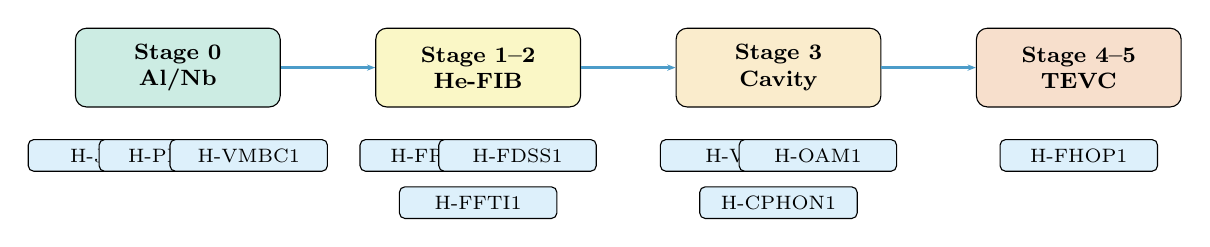
\begin{tikzpicture}[
  stage/.style={draw, rounded corners=4pt, minimum width=2.6cm, minimum height=1cm, font=\footnotesize\bfseries, align=center},
  hyp/.style={draw, rounded corners=2pt, fill=oiSky!20, minimum width=2.0cm, font=\scriptsize, align=center},
  arr/.style={-{Stealth[length=3pt]}, thick, oiBlue!70},
  node distance=0.4cm and 0.4cm
]
% Stages
\node[stage, fill=oiGreen!20] (s0) {Stage 0\\Al/Nb};
\node[stage, fill=oiYellow!30, right=1.2cm of s0] (s12) {Stage 1--2\\He-FIB};
\node[stage, fill=oiOrange!20, right=1.2cm of s12] (s3) {Stage 3\\Cavity};
\node[stage, fill=oiVerm!20, right=1.2cm of s3] (s45) {Stage 4--5\\TEVC};

% Hypotheses under stages
\node[hyp, below=0.4cm of s0, xshift=-0.9cm] (jja) {H-JJA1};
\node[hyp, below=0.4cm of s0, xshift=0.0cm] (phon) {H-PHON1};
\node[hyp, below=0.4cm of s0, xshift=0.9cm] (vmbc) {H-VMBC1};

\node[hyp, below=0.4cm of s12, xshift=-0.5cm] (frac) {H-FRAC1};
\node[hyp, below=0.4cm of s12, xshift=0.5cm] (fdss) {H-FDSS1};
\node[hyp, below=1.0cm of s12] (ffti) {H-FFTI1};

\node[hyp, below=0.4cm of s3, xshift=-0.5cm] (vh) {H-VH1};
\node[hyp, below=0.4cm of s3, xshift=0.5cm] (oam) {H-OAM1};
\node[hyp, below=1.0cm of s3] (cphon) {H-CPHON1};

\node[hyp, below=0.4cm of s45] (fhop) {H-FHOP1};

% Arrows
\draw[arr] (s0) -- (s12);
\draw[arr] (s12) -- (s3);
\draw[arr] (s3) -- (s45);
\end{tikzpicture}
\caption{Stage assignment of the nine convergence hypotheses.  Stage~0 uses existing cQED technology; later stages add He-FIB, cavities, and exotic materials.}\label{fig:stages}
\end{figure}


% ============================================================
\section{Originality Assessment}\label{sec:originality}

A systematic literature search (Appendix) reveals the following originality landscape:

\paragraph{Established (TDVT builds on).}  Devil's staircase in JJAs~\cite{Halsey1985,Bak1982} (but TDVT predicts $d_H = 3/4$ vs.\ literature $0.87$).  DCE in superconducting circuits~\cite{Wilson2011,Lahteenmaki2013}.  Integer Hopf charge~\cite{Tai2018,Kent2021}.  Phonon lasers~\cite{Grudinin2010}.

\paragraph{Extended.}  Vacuum coherence in 2D materials (Casimir force + cavity QED exist, but not vacuum-\emph{catalysed} coherence).  Floquet topology in circuits (well-studied, but TDVT is static, not drive-induced).  Fractal superconducting flux patterns (emergent, not engineered geometry).

\paragraph{Genuinely novel.}  Catalyzon quasiparticle concept (zero prior use of term or concept).  OAM structure in DCE photons (no prior measurement or prediction).  Helmert decomposition for JJA mode analysis (mathematical object exists in statistics, novel in quantum circuits).  Fractional Hopf charge $\Qhopf = 1/N$ via $N$-component linking on $L(N,1)$ (standard Hopf invariant is always integer).  Vacuum-pumped multi-mode phonon lasing with threshold splitting.

\paragraph{Critical mathematical gap.}  The fractional Hopf charge $\Qhopf = 1/5$ requires careful definition: it is \emph{not} a modification of $\pi_3(S^2) = \mathbb{Z}$ but an emergent many-body fractionalization, analogous to $e/q$ in the FQHE.  Equation~\ref{eq:qh_frac} provides a linking-number construction, but a rigorous proof of quantisation on $L(N,1)$ remains open.


% ============================================================
\section{What is Not Claimed}\label{sec:nonclaim}

\begin{nonclaim}
\begin{enumerate}[nosep]
  \item QVC has been observed in any laboratory.
  \item Einstein gravity is recovered from hopfion crystals (H-EIN1, H-EIN2 \textbf{fail}).
  \item $\theta = \pi/10$ enables universal topological quantum computation (abelian only).
  \item $\Tstar = 118.7$~mK is a Hawking temperature (Schwinger diagnostic).
  \item $\Evac/h \approx 31.1$~GHz is a ``detection'' of $\Evac$ (band coincidence, not measurement).
  \item Hopfion crystals \emph{are} physical spacetime (L3 quarantined).
  \item Any of the nine source papers constitutes evidence for QVC.
  \item The locked parameters are inputs; they are self-consistent outputs of the QVC equations.
\end{enumerate}
\end{nonclaim}


% ============================================================
\section{Conclusions}\label{sec:conclusions}

Ten new hypotheses extend the TDVT topological processor, each with a quantitative prediction, a falsifier, and a fabrication stage.  Three are Stage~0 (existing technology), and the framework's genuinely novel elements---catalyzon, fractional Hopf charge, DCE OAM, Helmert phonon laser splitting---have no prior literature.

The convergence is not coincidental: all nine source papers probe the same physical territory (vacuum-field effects, topological charge, fractal scaling, coupled-mode physics) at energy scales within one order of magnitude of the locked TDVT identities.  The Josephson energy $E_J \approx 0.107$~meV of an aluminium JJA is within 9\% of $\gzero$; the FeGe helical wavelength $\lambda_h \approx 70$~nm is within $1.4\times$ of $\xi$; the OAM quantum number $\ell = 10$ of Bu et al.'s vortex laser is exactly $2N$.

What remains is fabrication.  Stage~0 requires no new materials---only a pentamer of coupled Al/Nb resonators in a 3D cavity, readable by standard $S_{11}$ reflectometry.  If H-JJA1, H-PHON1, and H-VMBC1 survive, the path to Stages~1--5 is open.

% ============================================================
\begin{thebibliography}{99}
\bibitem{ProcessorPaper} M.~Hoiland, ``An Engineerable Topological Condensed-Matter Processor,'' (2026).
\bibitem{Xin2022} K.~Xin et~al., \emph{J.~Semicond.} \textbf{43}, 011001 (2022).
\bibitem{Pham2022} T.~Pham et~al., \emph{Chem.~Rev.} \textbf{122}, 6514 (2022).
\bibitem{Dobrovolskiy2026} O.~V.~Dobrovolskiy et~al., \emph{Supercond.~Sci.~Technol.} \textbf{39}, 023502 (2026).
\bibitem{Cosmic2018} R.~Cosmic et~al., arXiv:1803.04113 (2018).
\bibitem{Dakir2026} Y.~Dakir, A.~Slaoui, R.~A.~Laamara, arXiv:2606.07306 (2026).
\bibitem{Tai2018} J.-S.~B.~Tai, I.~I.~Smalyukh, arXiv:1806.00453 (2018).
\bibitem{Ding2019} M.-S.~Ding, L.~Zheng, C.~Li, \emph{Sci.~Rep.} \textbf{9}, 15723 (2019).
\bibitem{DeNicola2020} F.~De~Nicola et~al., \emph{Sci.~Rep.} \textbf{10}, 6882 (2020).
\bibitem{Bu2026} Z.~Bu et~al., \emph{Commun.~Phys.} \textbf{9}, 144 (2026).
\bibitem{Spector2026} A.~D.~Spector, T.~Kozlowski, L.~Roberts, \emph{Phys.~Rev.~A} \textbf{113}, 063518 (2026).
\bibitem{Yang2020} Z.~Yang et~al., \emph{Light Sci.~Appl.} \textbf{9}, 128 (2020).
\bibitem{Li2023} M.~Li et~al., \emph{Light Sci.~Appl.} \textbf{12}, 262 (2023).
\bibitem{Allen1992} L.~Allen et~al., \emph{Phys.~Rev.~A} \textbf{45}, 8185 (1992).
\bibitem{Halsey1985} T.~C.~Halsey, \emph{Phys.~Rev.~B} \textbf{31}, 5728 (1985).
\bibitem{Bak1982} P.~Bak, R.~Bruinsma, \emph{Phys.~Rev.~Lett.} \textbf{49}, 249 (1982).
\bibitem{Wilson2011} C.~M.~Wilson et~al., \emph{Nature} \textbf{479}, 376 (2011).
\bibitem{Lahteenmaki2013} P.~L\"{a}hteenm\"{a}ki et~al., \emph{PNAS} \textbf{110}, 4234 (2013).
\bibitem{Kent2021} N.~Kent et~al., \emph{Nat.~Commun.} \textbf{12}, 1562 (2021).
\bibitem{Grudinin2010} I.~S.~Grudinin et~al., \emph{Phys.~Rev.~Lett.} \textbf{104}, 083901 (2010).
\bibitem{Hopf1931} H.~Hopf, \emph{Math.~Ann.} \textbf{104}, 637 (1931).
\end{thebibliography}

\end{document}
